% This is LLNCS.DOC the documentation file of
% the LaTeX2e class from Springer-Verlag
% for Lecture Notes in Computer Science, version 2.4
\documentclass{llncs}
\usepackage{llncsdoc}
\usepackage{graphicx}
%
\begin{document}

\title{CIT Brains @Home\\2016 Team Description Paper}

\author{Ryuichi Ueda \and
Yasuo Hayashibara \and
Shinya Fujie \and
Yuya Aoki \and
Hirofumi Inoue \and
Hiroto Matsuzaki \and
Kazuya Natsusako \and
Akie Ohno \and
Yuki Sato \and
Ryo Shimomura \and
Shotaro Terato \and
Kiyoshi Irie
}

\institute{Chiba Institute of Technology,\\
2-17-1 Tsudanuma, Narashino, Chiba, Japan\\
{\tt ryuichi.ueda@p.chibakoudai.jp\\
http://at-home.cit-brains.net/}}

\maketitle
%
\begin{abstract}
CIT Brains @Home has been newly set up in November 2015
as a derivational team from the world-champion team
in the humanoid league and from a team that participates in
an outdoor mobile robot competition in Japan.
Through participation in @Home league,
we contribute actively to the study of natural decision making
in home environments and to packaging of our past/future
software/hardware as reusable and open ones.
\end{abstract}

\section{The team}

CIT Brains @Home has been newly set up in November 2015
by the staff and students in Department of Advanced Robotics,
Chiba Institute of Technology.
The aim of this team is integration and presentation
of research progresses in our department.

Our team is made up of three (associate) professors and
one researcher, and eight graduate/undergraduate students.
Each background of the staff is as follows.
\begin{itemize}
	\item \textbf{Prof. Yasuo Hayashibara}
		takes care of manipulation and hardware.
		He is also the owner of CIT Brains in Humanoid league. 
		The team is the champion of Humanoid KidSize Robot league
		in 2014 \cite{hayashibara2015} and 2015 \cite{hayashibara2016}.
		He also participated in the small size league and rescue
		real robot league. His team for the rescue league,
		Toin Pelicans, became a winner in RoboCup 2004 \cite{lima2005}.
	\item \textbf{Assoc. Prof. Shinya Fujie} is interested in speech recognition
		\cite{fujie2009,matsuyama2015} and provides direction for implementation
		of human-robot interaction.
	\item \textbf{Research Fellow Kiyoshi Irie} is interested in image processing and
		environmental recognition \cite{irie2013,irie2015}. He is also a member
		of CIT Brains in the humanoid league.
	\item \textbf{Assoc. Prof. Ryuichi Ueda} heads this team.
		He takes care of navigation and decision making \cite{ueda2015}.
		He consecutively participated in RoboCup Sony four-legged league
		(starndard platform league)
		from 2001 Seattle \cite{arai2002tdp}
		as a student to 2007 Atlanta as an assistant professor.
		His team, Team ARAIBO, earned podiums from RoboCup 2003 to 2005
		in the technical challenge of the league \cite{pagello2004,lima2005}.
\end{itemize}

In this paper, we describe our present preparation for
RoboCup 2016 and for further contribution in the league.
Our robot is introduced in Sec.~\ref{sec:robot}.
Our interest in science and technology is
described in Sec.~\ref{sec:contribution}.
We conclude this description paper in Sec.~\ref{sec:conclusion}.

\section{Robot}\label{sec:robot}
The robot, shown in Fig.~\ref{fig:robot},
is mainly composed of a commercial mobile robot,
two self-produced manipulators, and a head part that is composed of
a microphone and Microsoft Kinect.

\begin{figure}[h]
	\begin{center}
		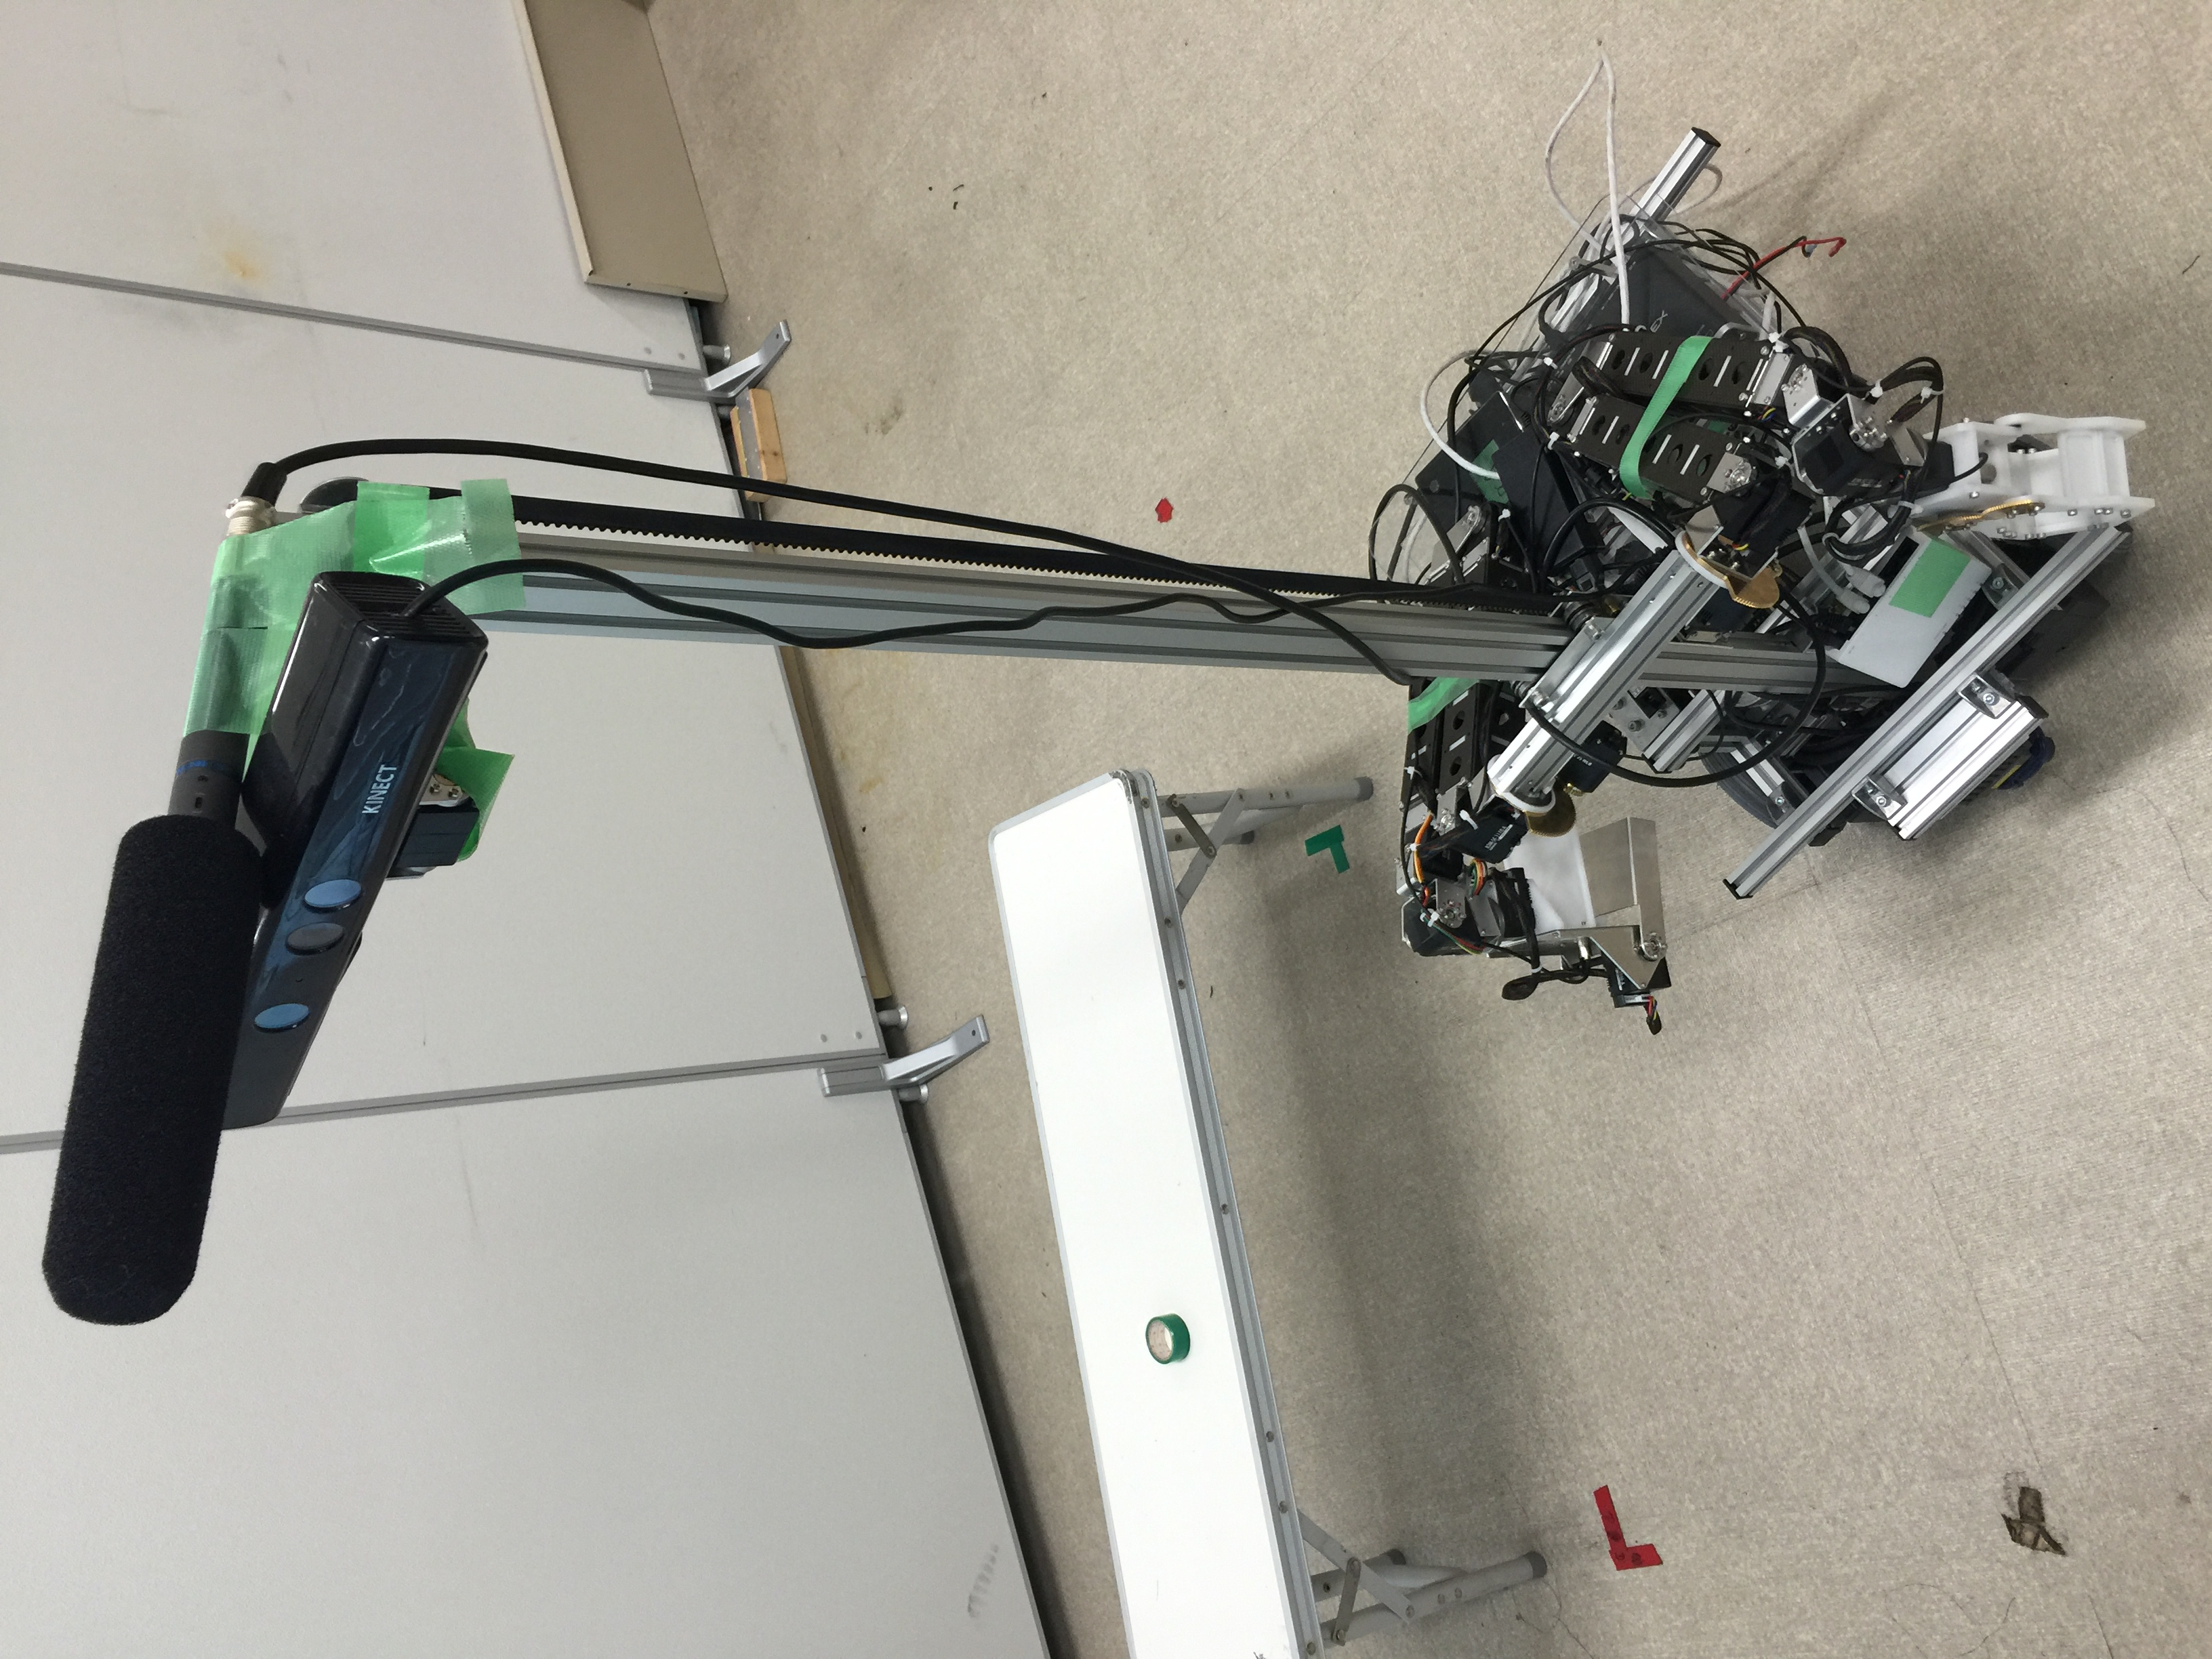
\includegraphics[width=0.6\linewidth]{./IMAGE/robot.eps}
		\caption{The robot (It has still no name.)}
		\label{fig:robot}
	\end{center}
\end{figure}

\subsection{Hardware}
\subsubsection{Mobile robot part}

We use i-Cart mini\cite{icartmini} as a mobile robot part
with some modifications. 
In our department, this robot is also used for Tsukuba Challenge,
which is an annual competition on outdoor navigation of mobile robots
held in Japan.
Our customized robot from i-Cart mini is named ORNE
(ORNE for Robot Navigation Engineers).

This mobile robot has two silent brushless motors.
Under the front bumper, an UTM-30LX-EW Scanning range finder
is attached for navigation.
Though these motors are very silent, 
they have an ability to make the robot move on public streets.
This mobile robot has two drive wheels whose diameter are 155[mm], 
and one rear caster whose diameter is 100[mm].
Each of the drive wheel is connected to a slient brushless motor.


\subsubsection{Head part}

A Microsoft Kinect at the top of the robot is used for
detecting and following persons.
For speech recognition, a directional microphone,
ATM57a made by audio-technica corporation, is attached
upon the Kinect.


\subsubsection{Manipulator part}

The robot has two arms and each arm has a hand.
They are shown in Fig.~\ref{fig:manipulators}.
We also give some movies in \cite{citba2016}.
The shapes of the left and right hands are different from each other.
The right hand, which equips two square plate for sandwiching,
is used for grabbing a snack bag or a round bottle.
The left hand can pinch an object with its tips,
or grab one with the inner side.
Figure~\ref{fig:joints} illustrates actuator arrangement of an arm.
The center part of the arm is composed of boxy assembled carbon plates
and acctuators that are arranged horizontally.
This lightweight structure ensures a large work space with small actuators.
This part is lifted and swung by the slider mechanism shown in
Fig.~\ref{fig:manipulator_attachment} and an actuator at the
root of the carbon part respectively.
They enlarge the work space, and make the robot enable to pick up
objects on the floor or higher parts of a shelf.


\begin{figure}[h]
	\begin{center}
		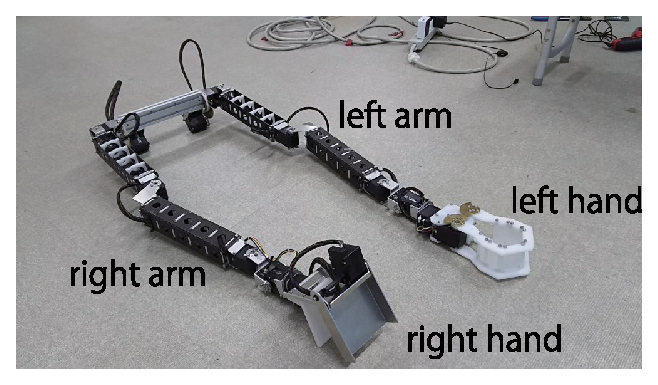
\includegraphics[width=0.7\linewidth]{./IMAGE/manipulators.eps}
		\caption{Manipulators and hands}
		\label{fig:manipulators}
	\end{center}
\end{figure}

\begin{figure}[h]
\begin{minipage}{23em}
	\begin{center}
		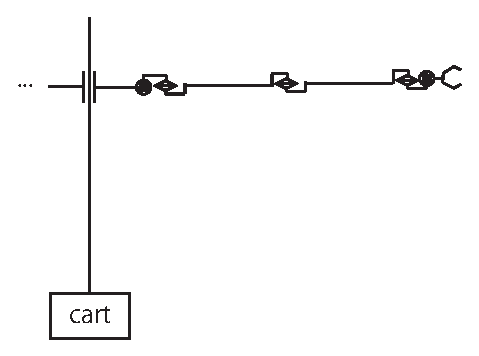
\includegraphics[width=0.95\linewidth]{./IMAGE/joints.eps}
		\caption{Joints of an arm}
		\label{fig:joints}
	\end{center}
\end{minipage}
\begin{minipage}{15em}
	\begin{center}
		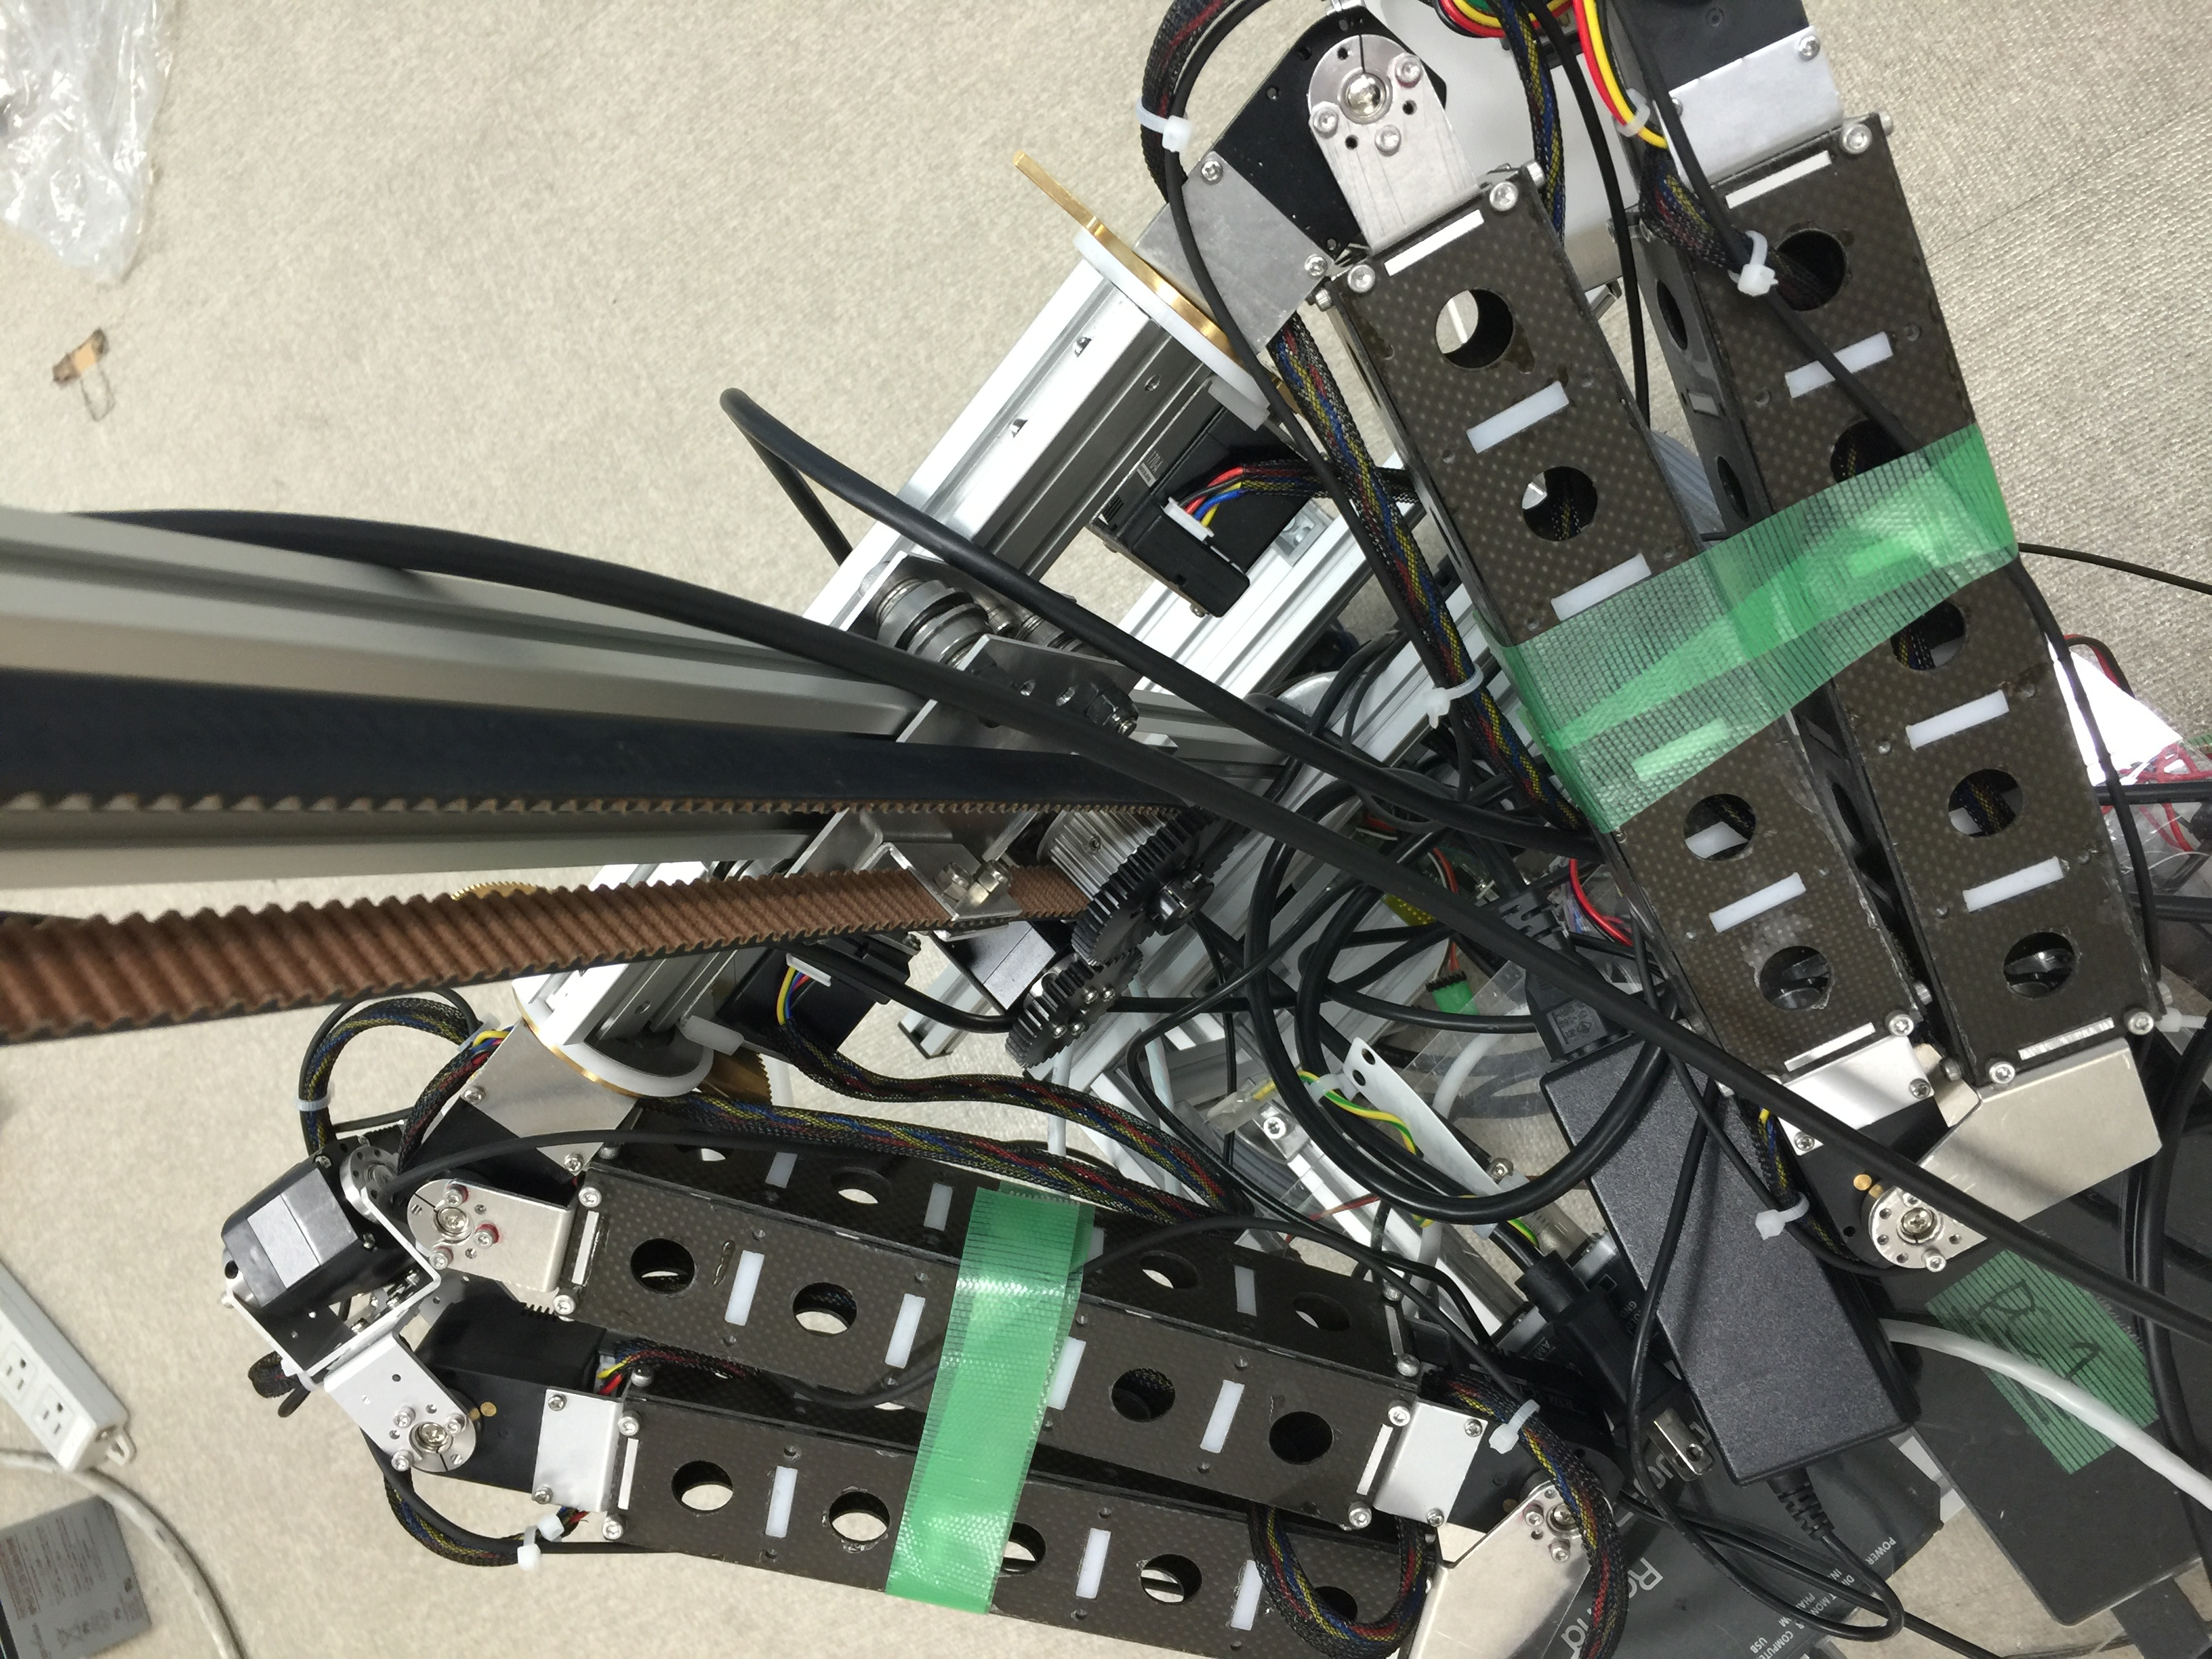
\includegraphics[width=0.95\linewidth]{./IMAGE/manipulator_attachment.eps}
		\caption{Attachment of Manipulators}
		\label{fig:manipulator_attachment}
\end{center}
\end{minipage}
\end{figure}

Each hand has a camera for object recognition.
An movie obtained with one of the cameras is shown in
\texttt{https://youtu.be/XInH9a2ISdA}.


\subsubsection{Cover of the robot} We have never been prepared.

\subsection{Computers and software}

\subsubsection{Collaboration of computers}
The robot has three computers. Decision making is done by
nodes of the robot operating system (ROS).
ROS runs on Ubuntu Linux 14.04 LTS, which works on
a GIGABYTE BRIX PC. A Windows note PC is used for processing
the data from Microsoft Kinect.
These two PCs exchange data via A Raspberry Pi.
The Ubuntu PC and the Windows PC push and pull
data with the rsync command.

We adopt this loose coupling structure
so as to reduce our workloads in the early stages.
Though the Ubuntu PC obtains each cycle of data from Kinect
after some delay, software for communication becomes
quite simple. This structure will be changed to
another tight structure if we must do it.


\subsubsection{ROS nodes}
Figure~\ref{fig:rqt_graph} shows the structure of ROS nodes.
Since we need to construct software in short term, 
we have reused nodes for Tsukuba Challenge (modules named
\texttt{orne\_...} in the figure).
The software for Tsukuba Challenge also contain open source nodes
(\texttt{move\_base,amcl...}) and nodes for i-Cart mini (\texttt{icart\_...}).

\begin{figure}[p]
	\begin{center}
		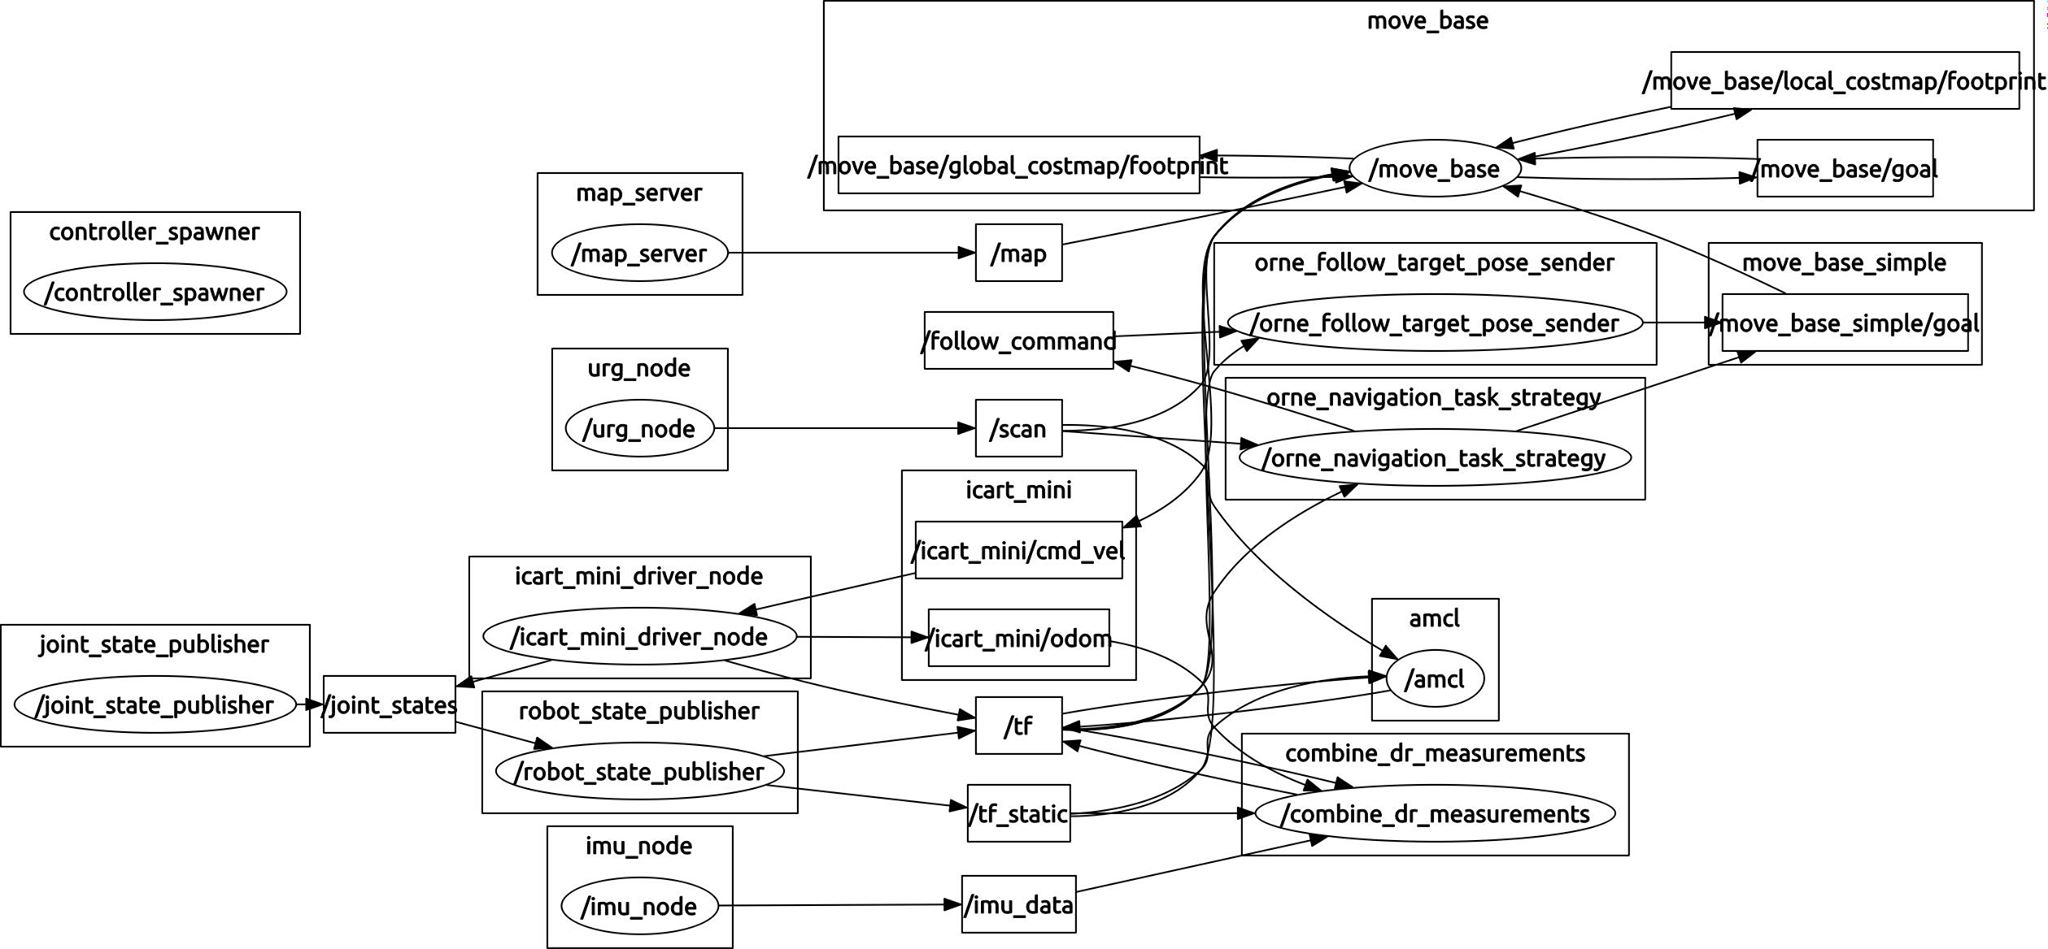
\includegraphics[width=0.8\linewidth]{./IMAGE/rqt_graph.eps}
		\caption{Output of rqt\_graph}
		\label{fig:rqt_graph}
	\end{center}
\end{figure}

\subsubsection{Main controller}
These reused nodes are controlled by
\texttt{orne\_navigation\_task\_strategy},
which is a simple Python script.
This module is presently specialized for
a subset problem of the navigation task.
The movie in which the robot works with this module
can be seen in \texttt{https://youtu.be/eR5cCLBpbFg}.

\subsubsection{Nodes for arms (in the planning stage)}
Nodes for the arms and hands are under construction and
they are not appeared in Fig.~\ref{fig:rqt_graph}.
We will utilize MoveIt! (\texttt{http://moveit.ros.org/})
for their control.

\subsection{Applicability of the robot in the real world}

To use this robot in a real home environment,
we need to make an outer package of this robot at first.
In this stage, we have checked motions of the mobile robot part
and the manipulator part separately.


\section{Innovative technology and scientific contribution}\label{sec:contribution}

\subsection{Scientific interest}

Our basic idea to realize home-care robots is that they
should try something even if they do not have certain information
what they should do. Some mistakes will occur when the robot
acts without certain information.
However, a decision making rule that permits mistakes will make
a robot accomplish more tasks than another rule that waits for
perfect information.

We also think that decision making with this loose policy
will generate a natural communication between a robot and its owners.
For example, when the owner asks his/her robot to bring cookies,
he/she wants to eat cookies with a high probability.
However, there is some some possibility that the owner
only wants to fill his/her stomach.
In the real life, there are some incidents
(e.g. a construction noise) that
makes the robot never be able to understand the word ``cookies.''
We think that the robot should start moving in that case
even if it does not have certain information.
Then it should receive feedback from the owner
by asking questions or by speculative behaviors.
Though these interactive processes are sometimes laborious,
we always do that so as to finish various tasks within
the time limits.

This idea is based on our study in a POMDP
(partially observable Markov decision process) problem
\cite{ueda2015}. In this study, problems defined in
simple state spaces that are spanned several state variables
are handled. We will tackle extension and application of
the algorithm to more complicated problems.


\subsection{Externally available components}

We have developed a ROS module for servo motors made
by Kondo Kagaku Co., Ltd.
as our first contribution\cite{hayashibara_kondo}.
We will publish our software through GitHub.

\section{Conclusion and future work}\label{sec:conclusion}

We have reported our present preparation for
RoboCup 2016 and for further contribution in the league.
As described in this paper, there are some unimplemented
hardware and software. However, we have build our hardware
and software in this four month with rapidity.

We participate in RoboCup JapanOpen 2016 in this March.
The outer package of the robot will be prepared before
this event. After that, we will devote concentrated effort
to software for each test.



\bibliographystyle{splncs03}
\bibliography{../bibfiles/eng,../bibfiles/url}

\end{document}
